\chapter{Redes dinâmicas}
 \label{chap:redes-dinamicas}
 % Clustering Dynamic Spatio-Temporal Patterns in the Presence of Noise and Missing Data: https://www.ijcai.org/Proceedings/15/Papers/365.pdf
 %TODO --- Introduzir o processo de previsão de agrupamentos espaço temporais ---
 
Para redes dinâmicas, o foco é tipicamente em uma classe de redes e em questões referentes às estrutura dessa classe de rede, como a estrutura evoluiu e como isso afeta sistemas dinâmicos na rede. As redes temporais normalmente são mais orientadas a dados - onde se investiga um conjunto de dados, suas estruturas e como, por exemplo, surtos epidêmicos se comportariam sobre ele \cite{holme:colloquium}.

Uma observação sobre endemias é que casos e focos destes tendem a estar mais próximos do que distantes no espaço e no tempo. Por exemplo, o casos de dengue de amanhã tem mais probabilidade de serem semelhantes aos casos de hoje do que de um mês atrás ou mais. Da mesma forma, os casos num raio de 300 metros tendem a ser mais semelhantes do que os casos a 10 quilômetros ou mais de distância. Estas observações são referidas como dependência temporal e espacial.

\section{Previsão e Predição Espaço-Temporal}

A aceitação de modelos espaço-temporais tem sido tradicionalmente limitada pela escassez de conjuntos de dados espaço-temporais em grande escala \cite{Griffith2010}. Essa situação foi revertida nas últimas décadas e com grande quantidade de dados exige-se métodos rápidos e eficazes para lidar com eles. Os modelos espaço-temporais podem ser divididos em duas categorias: métodos estatísticos ou paramétricos e métodos de aprendizagem de máquina ou não-paramétricos.


\section{Agrupamento de dados baseado em predição}

A tarefa de predição visa descobrir o valor futuro de um determinado atributo de dados. É uma área com variedade de aplicações em diversas campos do conhecimento como meteorologia e detecção de doenças. Por exemplo, um médico gostaria de prever a reação de seus pacientes a um novo medicamento para diabetes, particularmente a duração dos episódios de hipoglicemia.

Na previsão de eventos é desejável prever a ocorrência de um evento ou o número de ocorrências de um evento ou a duração de um evento, dada a existência de certas condições. Por exemplo, um médico acaba de colocar um de seus pacientes epilépticos em uma nova droga que é muito eficaz, mas após o início da terapia pode causar um grave ataque de enxaqueca. O médico gostaria de prever a duração desse ataque, considerando o conhecimento sobre a idade do paciente e o número e duração dos ataques epilépticos no último ano. Nos problemas de previsão de eventos que lidam com a previsão da duração de um evento pode ser modelada usando uma variável contínua e pode-se usar a regressão linear para sua previsão, onde a regressão linear é um dos métodos de regressão mais amplamente disponíveis \cite{Mitsa:2010}.

Na previsão de séries temporais, os dados são informações históricas obtidas em intervalos de tempo regulares. Informações sobre padrões passados podem ser usadas para prever padrões futuros. No exemplo da enxaqueca, os dados poderiam ser a duração dos ataques de enxaqueca de outros pacientes sobre a droga, juntamente com informações sobre suas idades, condições médicas preexistentes e gravidade da epilepsia.

\section{Método de Lahiri}
\label{lahiri}
\citeautoronline{lahiri2007} apresentam um algoritmo de predição em redes temporais, e que usa a ideia de que certas interações sinalizam a ocorrência de outros em algum momento no futuro. Através de análises estatísticas o algoritmo mede o atraso entre as interações, e com isso pode-se prever quando certas interações vão ocorrer com base em observações passadas e atuais. Propõe-se a utilização de subgrafos frequentes e discute como identificar subgrafos que persistem em redes temporais.

\citeautoronline{lahiri2008} em seguida propõe um novo problema de mineração de dados para redes dinâmicas: detecção de todos os padrões de interação que ocorrem em intervalos de tempo regulares.

\section{O modelo Dynagraph}

A representação dos dados de indivíduos no espaço-tempo é muito importante, para que também se possa acompanhar a solução obtida pelos métodos de agrupamento estudados. O Dynagraph \cite{dynagraph} é um modelo computacional que permite, a partir de uma estrutura de dados simples, modelo de um Grafo ou Rede Dinâmica, representar com o mínimo custo de armazenamento a evolução de uma instância de observação e estudos. Ele acompanha a evolução dos conjuntos de um grafo: de nós e ligações (arcos e elos), como inserção/retirada ao longo do tempo, e mudança de suas características (posição, cor, forma, tamanho, e outras), por meio de um Editor de Características.

Trata-se de um poderoso instrumento de visualização e representação de eventos discretos espaço-temporais em mapas geográficos bidimensionais, que permite incorporar recursos de agrupamentos, predições e previsões de eventos que são discretizados numa determinada medida de intervalos temporais (segundos, minutos, horas, dias, semanas, decêndios, quinzenas, meses, anos).

\subsection{Estrutura de Dados}

A estrutura de dados usada no Dynagraph segue a notação de Objeto Javascript (\acrfull{JSON}), que é um formato de texto de intercâmbio de dados \cite{douglas}. A figura \ref{fig:jsondynagraph} mostra como é essa estrutura seguindo três objetos principais: ``metadata'', ``binding'' e ``data''.

Em ``metadata'' são definidos os campos para utilização de qualquer identificador, por exemplo: é possível utilizar ``ini'' e ``fim'',
que representam o tempo inicial e final de um elemento, no lugar de ``start'' e ``end'' respectivamente.

Na figura \ref{fig:jsondynagraph}, em ``binding'' são definidas as características dos vértices e arestas.

Seguindo o exemplo da mesma figura, ``vertex'' poderá
ser do tipo ``v1'', ``v2'' e ``v3'', onde cada tipo contém informações da forma do vértice. Essa forma pode ser uma imagem no formato
``png'' ou ``jpg'' ou customizada com as seguintes características:
\begin{itemize}
\item path: círculo ou seta;
\item fillColor: cor do preenchimento;
\item strokeColor: cor da borda;
\item fillOpacity: opacidade;
\item scale: tamanho;
\item strokeWeight: espessura da borda.
\end{itemize}

A aresta, ou ``polyline'', segue uma estrutura semelhante à do ``vertex'', porém com algumas particularidades como repetição de um símbolo
ao longo da aresta, e uma customização no campo ``path'' seguindo a notação SVG\footnote{\label{note} Scalable Vector Graphics - é uma forma de descrever de forma vetorial desenhos e gráficos bidimensionais}.

Em ``data'' são definidos os elementos do grafo, os tempos de início e fim de cada elemento ou tempo de existência. No caso dos vértices, a posição de cada elemento pode ser escrita no formato \acrshort{UTM} (\acrlong{UTM}) ou latitude e longitude.
O tipo de cada elemento, descrito em ``binding'', e no caso das arestas, são definidos os pontos de origem e destino.

Na figura \ref{fig:jsondynagraph} vemos a estrutura de construção de um grafo dinâmico. Os campos ``metadata'' e ``binding'' foram omitidos para evidenciar o objeto ``data''.
\FloatBarrier
\lstinputlisting[language=Java, basicstyle=\tiny]{figuras/new.json}
\begin{figure}[!htbp]
  \caption{Estrutura JSON usada pelo Dynagraph}
  \label{fig:jsondynagraph}
\end{figure}

\subsection{Editor de Características}

O Editor de Características é uma extensão do software Dynagraph. Ele permite alterar os atributos visuais dos vértices e aresta de um grafo dinâmico. Com ele pode-se criar novos tipos de dados e com isso diferenciar, por exemplo, focos de casos de dengue e tipos de dengue.
Essa extensão permite criar com os seguintes atributos: Rótulo, Opacidade, Escala, Espessura da Borda, Cor da Borda e Cor de Preenchimento. Outra opção é utilizar uma imagem.
 
A figura \ref{fig:edCaMenu} exibe a localização do Editor de Características na aplicação em um menu lateral com as seguinte opções: Vértice, Aresta e um painel, este exibe a data atual e número de vértices e arestas em análise.
\begin{figure}[!ht]
	\centering	
	\caption{\label{fig:edCaMenu} Editor de Características: menu lateral}
	\UECEfig{}{
		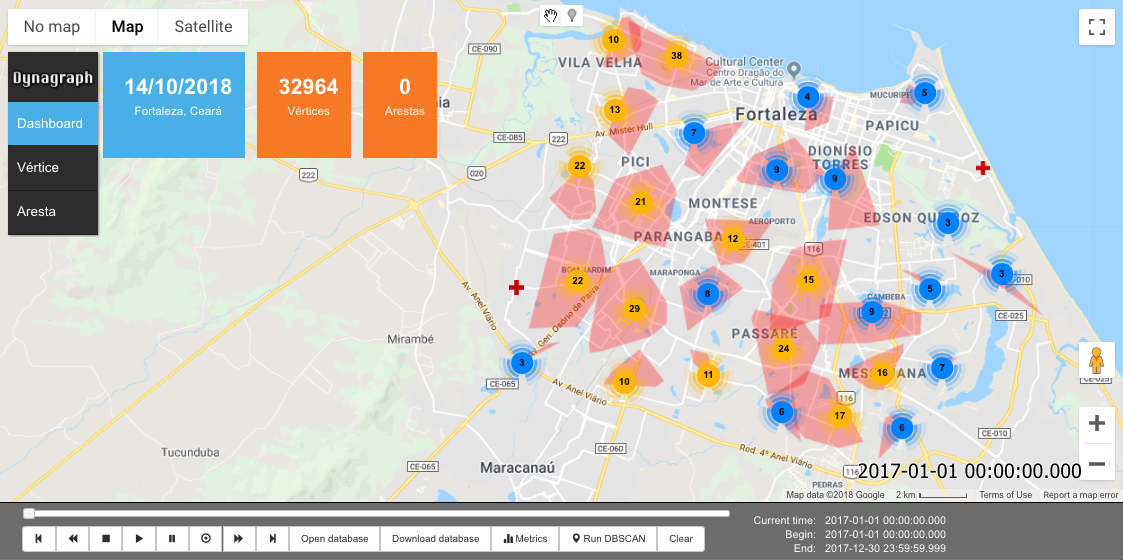
\includegraphics[width=15cm]{figuras/editorCaract/edCaractMenu.png}
	}{
		\Fonte{Elaborado pelo autor}
	}
\end{figure}
\FloatBarrier

Para criar um novo vértice, deve-se selecionar o submenu relacionado a vértices como mostra a figura \ref{fig:edCaCriacao1}.
\begin{figure}[!ht]
	\centering	
	\Caption{\label{fig:edCaCriacao1} Editor de Características: criação de um vértice}	
	\UECEfig{}{
		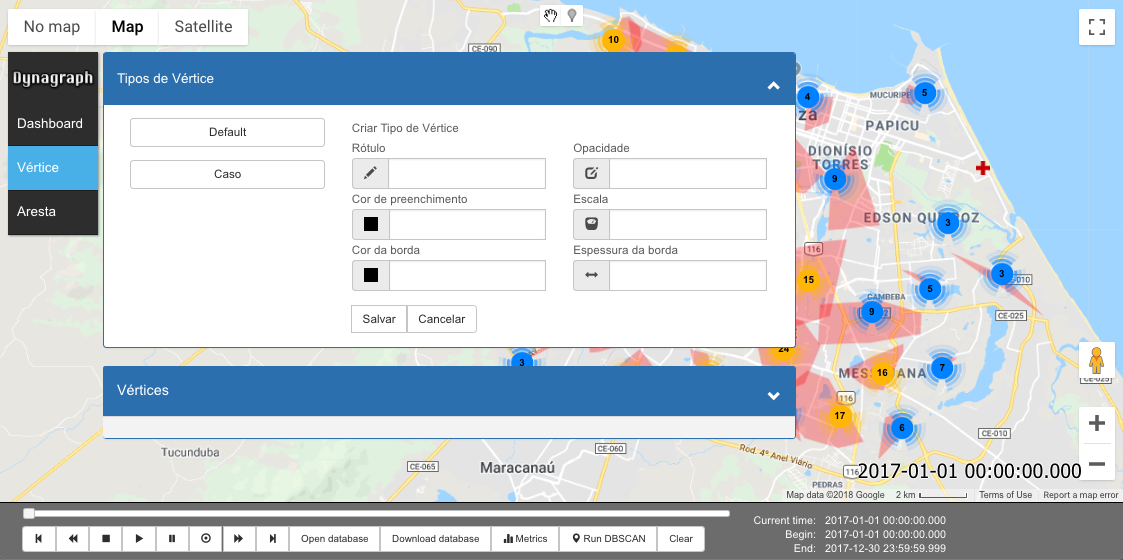
\includegraphics[width=15cm]{figuras/editorCaract/1edCaractCreateVertice.png}
	}{
		\Fonte{Elaborado pelo autor}
	}
\end{figure}
\FloatBarrier

A figura \ref{fig:edCaCriacao2} exibe os tipos de dados permitidos na criação ou edição de um vértice.
\begin{figure}[!ht]
	\centering	
	\Caption{\label{fig:edCaCriacao2} Editor de Características: criação de um vértice - tipos de dados}	
	\UECEfig{}{
		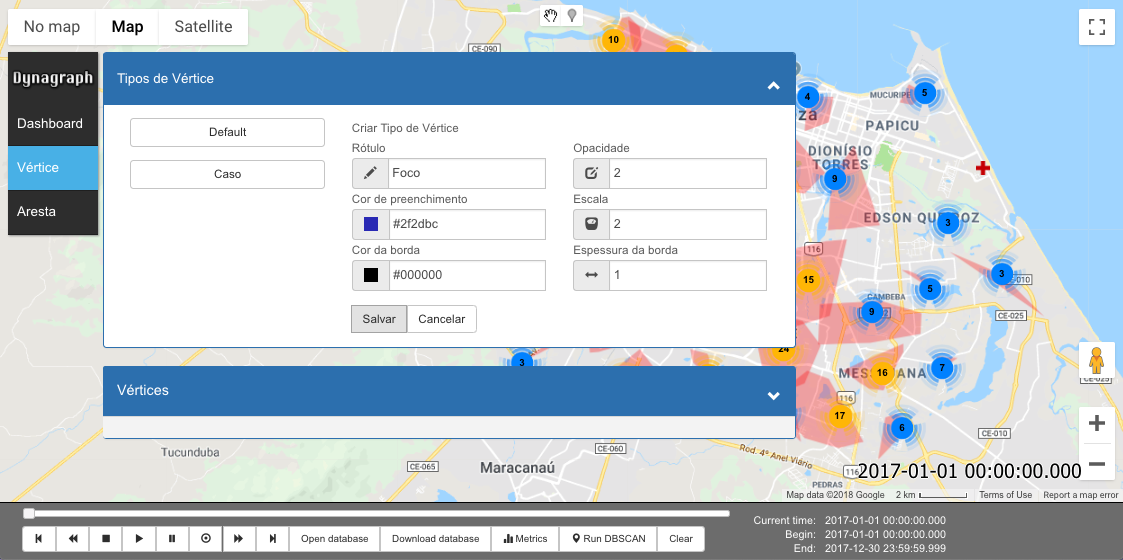
\includegraphics[width=15cm]{figuras/editorCaract/2edCaractCreateVertice.png}
	}{
		\Fonte{Elaborado pelo autor}
	}
\end{figure}
\FloatBarrier

Após criar um novo tipo de vértice é possível usá-lo editando um dado ponto no mapa, como mostram as figuras \ref{fig:edCaChangeV1} e \ref{fig:edCaChangeV2}. A figura \ref{fig:edCaShowV} exibe o resultado esperado.
\begin{figure}[!ht]
	\centering	
	\Caption{\label{fig:edCaChangeV1} Editor de Características: edição de um vértice - parte 1}	
	\UECEfig{}{
		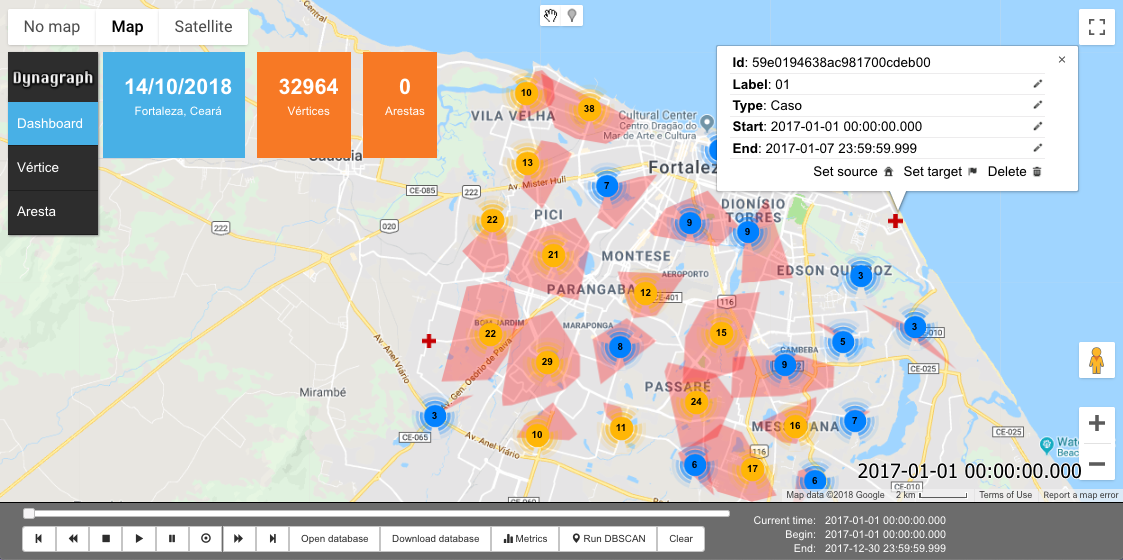
\includegraphics[width=15cm]{figuras/editorCaract/3edCaractChangeVertice.png}
	}{
		\Fonte{Elaborado pelo autor}
	}
\end{figure}
\FloatBarrier

\begin{figure}[!ht]
	\centering	
	\Caption{\label{fig:edCaChangeV2} Editor de Características: edição de um vértice - parte 2}	
	\UECEfig{}{
		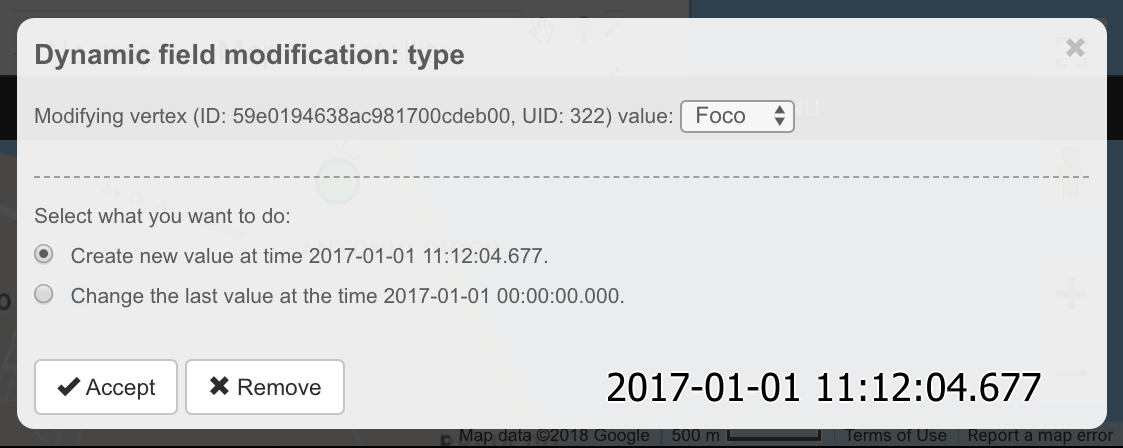
\includegraphics[width=15cm]{figuras/editorCaract/4edCaractChangeVertice.png}
	}{
		\Fonte{Elaborado pelo autor}
	}
\end{figure}
\FloatBarrier

\begin{figure}[!ht]
	\centering	
	\Caption{\label{fig:edCaShowV} Editor de Características: edição de um vértice - parte 3}	
	\UECEfig{}{
		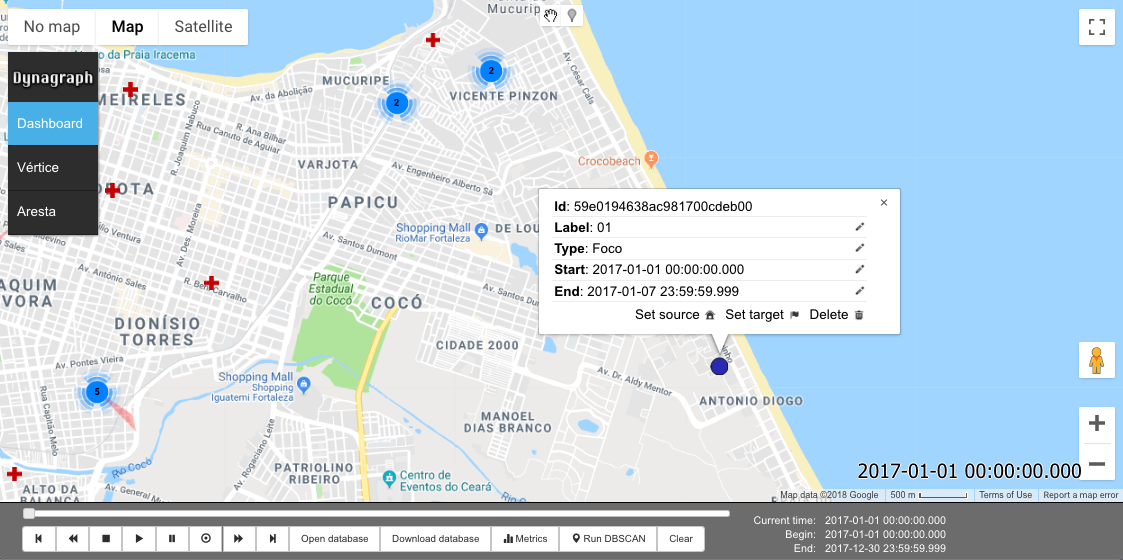
\includegraphics[width=15cm]{figuras/editorCaract/5edCaractShowVertice.png}
	}{
		\Fonte{Elaborado pelo autor}
	}
\end{figure}
\FloatBarrier

Para editar um tipo de vértice basta selecioná-lo a partir da lista de tipos de vértices e então aplicar as mudanças, como mostra a figura \ref{fig:edCaEditV1} e o resultado na figura \ref{fig:edCaEditV2}.
\begin{figure}[!ht]
	\centering	
	\Caption{\label{fig:edCaEditV1} Editor de Características: edição de um tipo de vértice - parte 1}	
	\UECEfig{}{
		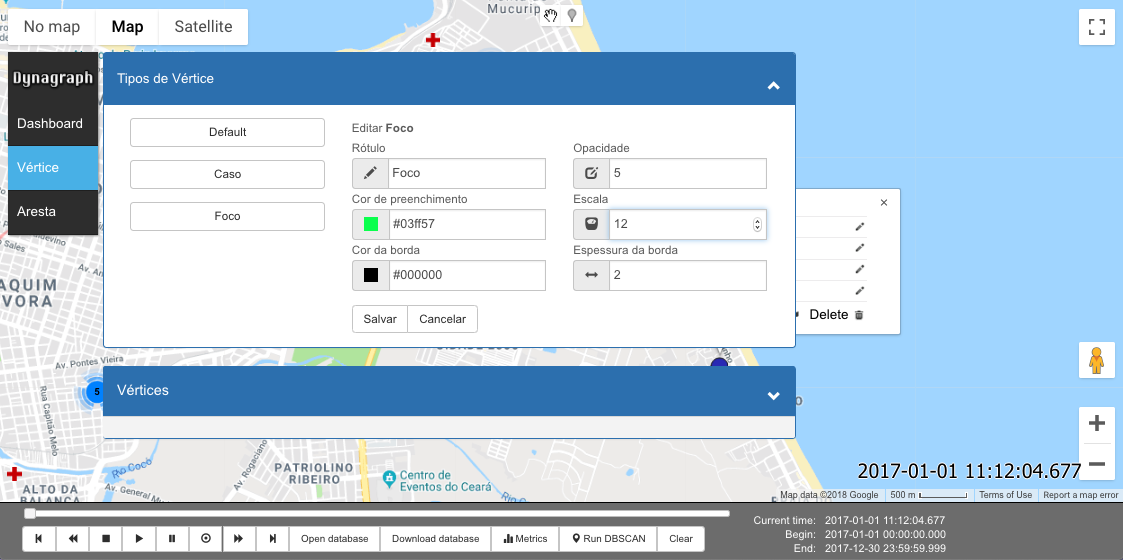
\includegraphics[width=15cm]{figuras/editorCaract/6edCaractEditVertice.png}
	}{
		\Fonte{Elaborado pelo autor}
	}
\end{figure}
\FloatBarrier
\begin{figure}[!ht]
	\centering	
	\Caption{\label{fig:edCaEditV2} Editor de Características: edição de um tipo de vértice - parte 2}	
	\UECEfig{}{
		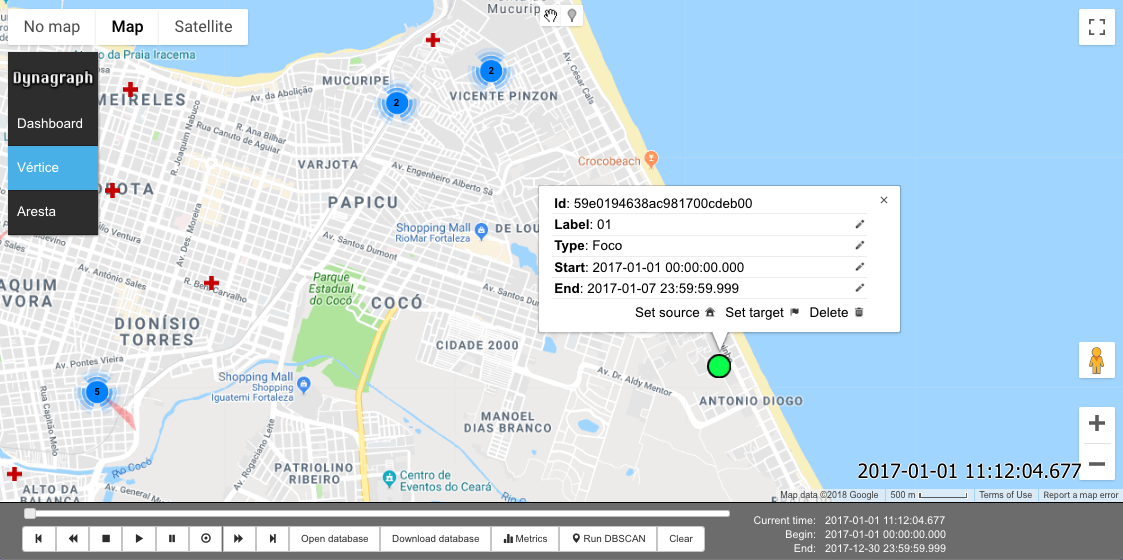
\includegraphics[width=15cm]{figuras/editorCaract/7edCaractEditedVertice.png}
	}{
		\Fonte{Elaborado pelo autor}
	}
\end{figure}
\FloatBarrier

Outra opção de edição de um vértice é dada na figura \ref{fig:edCaractEditVerticeOption2}. Nesta opção pode-se usar uma imagem pronta.
\begin{figure}[!ht]
	\centering	
	\Caption{\label{fig:edCaractEditVerticeOption2} Editor de Características: Tipo de vértice}	
	\UECEfig{}{
		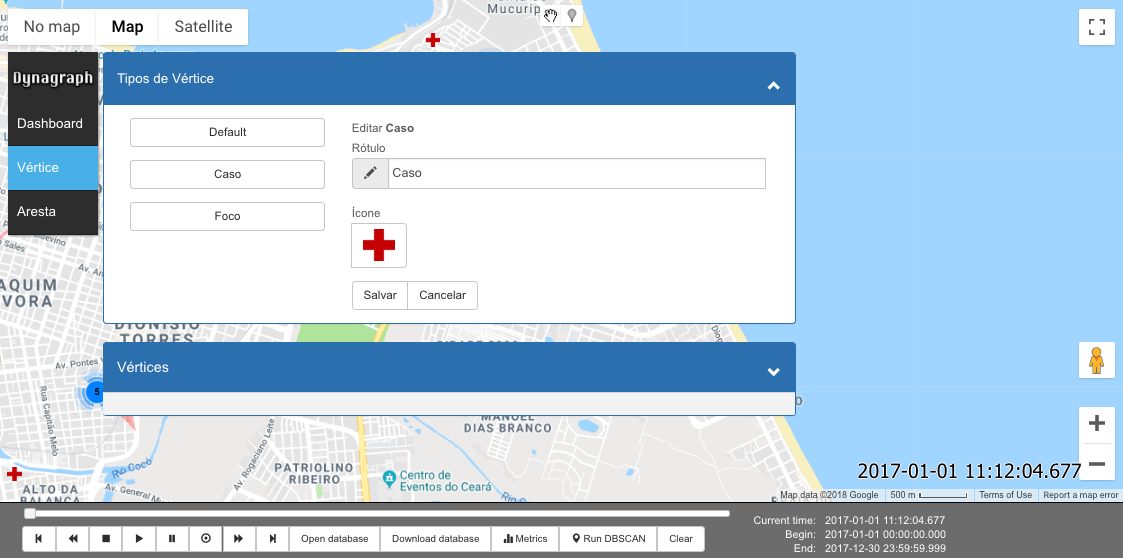
\includegraphics[width=15cm]{figuras/editorCaract/edCaractEditVerticeOption2.png}
	}{
		\Fonte{Elaborado pelo autor}
	}
\end{figure}
\FloatBarrier

O Editor de Características permite também a criação e edição de arestas (figura \ref{fig:edCaractAresta}), mas essa funcionalidade não foi necessária nesta pesquisa.
\begin{figure}[!ht]
	\centering	
	\Caption{\label{fig:edCaractAresta} Editor de Características: Aresta}	
	\UECEfig{}{
		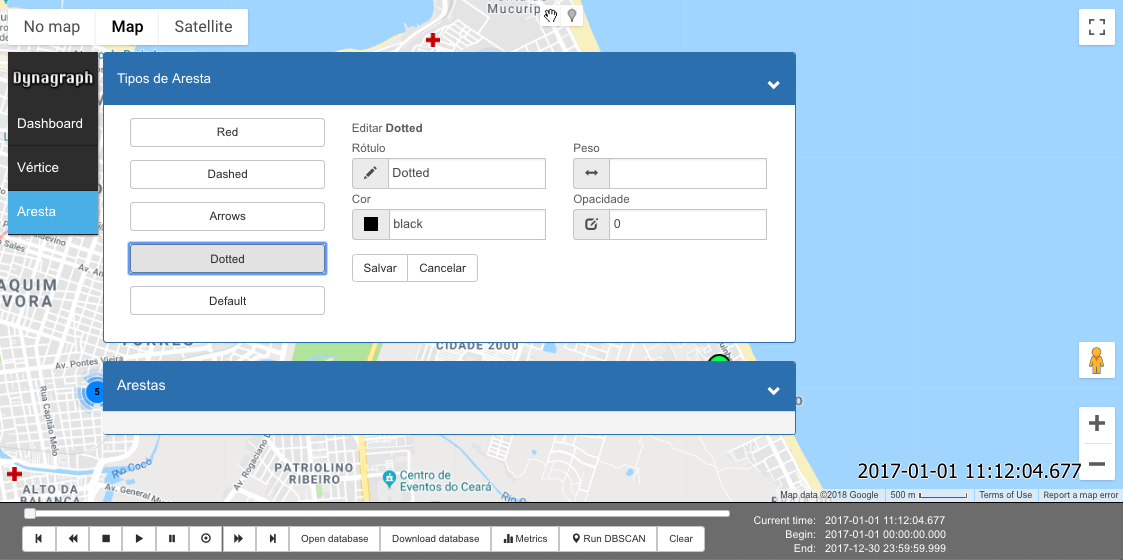
\includegraphics[width=15cm]{figuras/editorCaract/edCaractAresta.png}
	}{
		\Fonte{Elaborado pelo autor}
	}
\end{figure}
\FloatBarrier

\subsection{Visualização dos grupos formados}

Foram usados dois algoritmos para permitir a visualização dos grupos formados em um dado tempo. O primeiro é proveniente de uma biblioteca de \acrshort{API}s do Google chamada \emph{MarkerClusterer} \cite{markerCluster}, que cria e gerencia grupos de acordo com o nível de \textit{zoom} para grandes quantidades de pontos. Essa biblioteca é combinada com a \acrshort{API} Javascript do Google Maps$^{TM}$ para agrupar os pontos por proximidade e simplificar a exibição dos pontos no mapa.
De acordo com o nível de \textit{zoom} os grupos são formados com cores e tamanhos diferentes, como mostram as figuras \ref{fig:apiGoogleMaps1} e \ref{fig:apiGoogleMaps2}.
\begin{figure}[!ht]
	\centering	
	\Caption{\label{fig:apiGoogleMaps1} Grupos - \acrshort{API} Google Maps parte 1}	
	\UECEfig{}{
		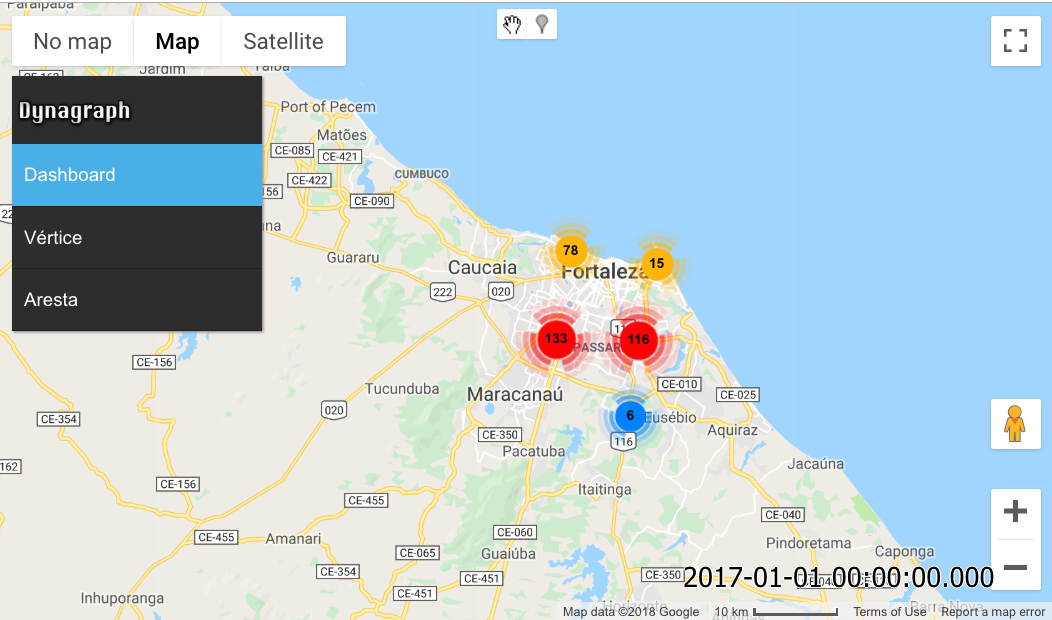
\includegraphics[width=13cm]{figuras/ClusterAPIGoogle1.png}
	}{
		\Fonte{Elaborado pelo autor}
	}
\end{figure}
\FloatBarrier

\begin{figure}[!ht]
	\centering	
	\Caption{\label{fig:apiGoogleMaps2} Grupos - \acrshort{API} Google Maps parte 2}	
	\UECEfig{}{
		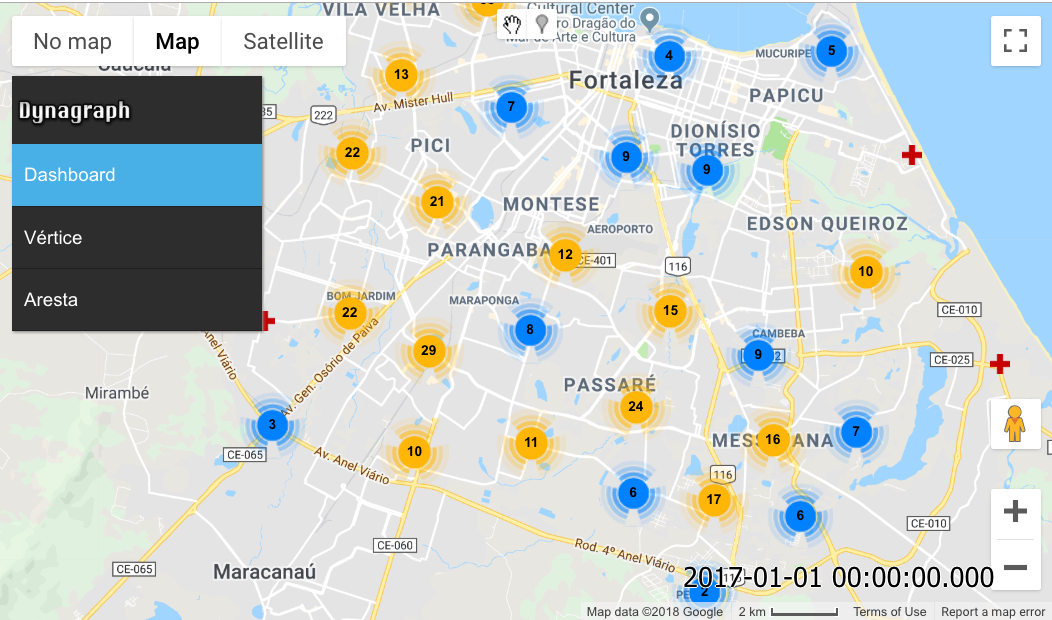
\includegraphics[width=13cm]{figuras/ClusterAPIGoogle2.png}
	}{
		\Fonte{Elaborado pelo autor}
	}
\end{figure}
\FloatBarrier

O segundo algoritmo é conhecido como {\em Convex Hull} \cite{ConvexHull}. Também denominado de fecho convexo ou envoltória convexa. No problema é dado um conjunto de pontos no espaço Euclideano e deseja-se encontrar o menor número de pontos que geram um polígono convexo no qual abranja todos os outros pontos.
As figuras \ref{fig:algConvexHull1} e \ref{fig:algConvexHull2} apresentam exemplos do \emph{convex hull}, onde cada polígono representa o grupo de casos humanos de dengue naquela região delimitada. Dos vários pontos, somente os pontos mais externos é que formam o menor polígono que engloba todos os outros pontos.
%
\begin{figure}[!ht]
	\centering	
	\Caption{\label{fig:algConvexHull1} Exemplo 1 de Convex Hull}	
	\UECEfig{}{
		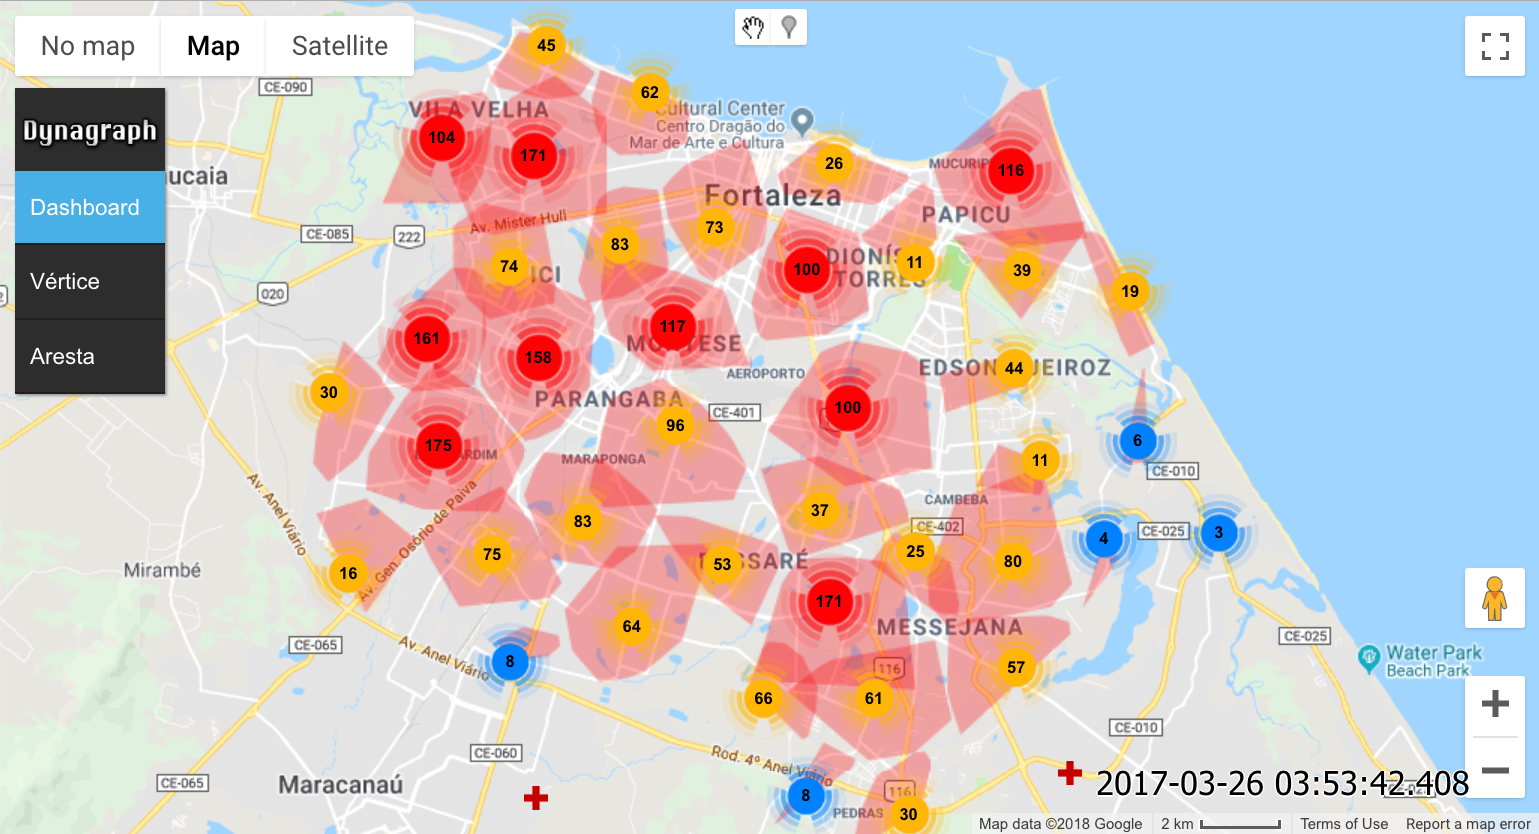
\includegraphics[width=14cm]{figuras/algConvexHull1.png}
	}{
		\Fonte{Elaborado pelo autor}
	}
\end{figure}
\FloatBarrier
\begin{figure}[!ht]
	\centering	
	\Caption{\label{fig:algConvexHull2} Exemplo 2 de Convex Hull}	
	\UECEfig{}{
		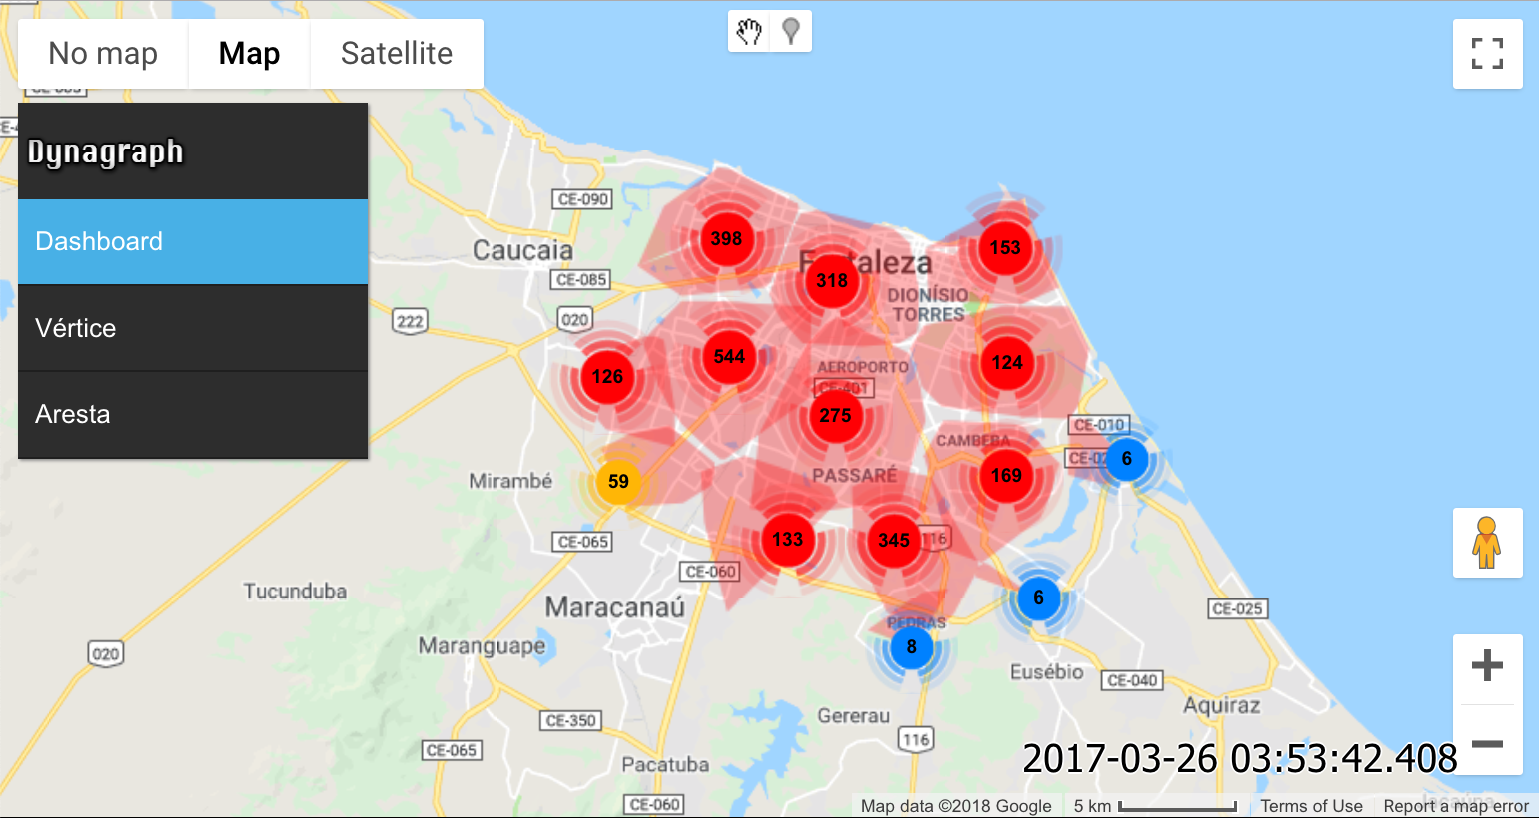
\includegraphics[width=14cm]{figuras/algConvexHull2.png}
	}{
		\Fonte{Elaborado pelo autor}
	}
\end{figure}
\FloatBarrier

\subsection{Banco de Dados Multidimensional}
Bancos de dados espaço-temporais armazenam informações sobre as posições de objetos individuais ao longo do tempo. Em muitas aplicações, no entanto, como sistemas de monitoramento de endemias, são necessários apenas dados resumidos, como o número médio de casos de dengue em uma área por um período específico.
Em \cite{Papadias2002}, os autores descrevem a construção de um Armazém de Dados (\acrshort{DW} - \textit{\acrlong{DW}}) espaço-temporal que suporta operações \acrshort{OLAP} - \acrlong{OLAP}. Os dados \acrshort{OLAP} são armazenados em cubos, em vez de tabelas e essa estrutura multidimensional fornece acesso rápido a dados para análise, permitindo manipular e visualizar os dados, para que possa extrair as informações relevantes \cite{faghmous2013}, \cite{Mitsa:2010}. Os dados espaço-temporais usados no Dynagraph são armazenados individualmente e as consultas abordam pontos espaço-temporais individuais. A figura \ref{fig:olap} representa esse banco de dados multidimensional.

\begin{figure}[!ht]
	\centering	
	\Caption{\label{fig:olap} Cubo OLAP}	
	\UECEfig{}{
		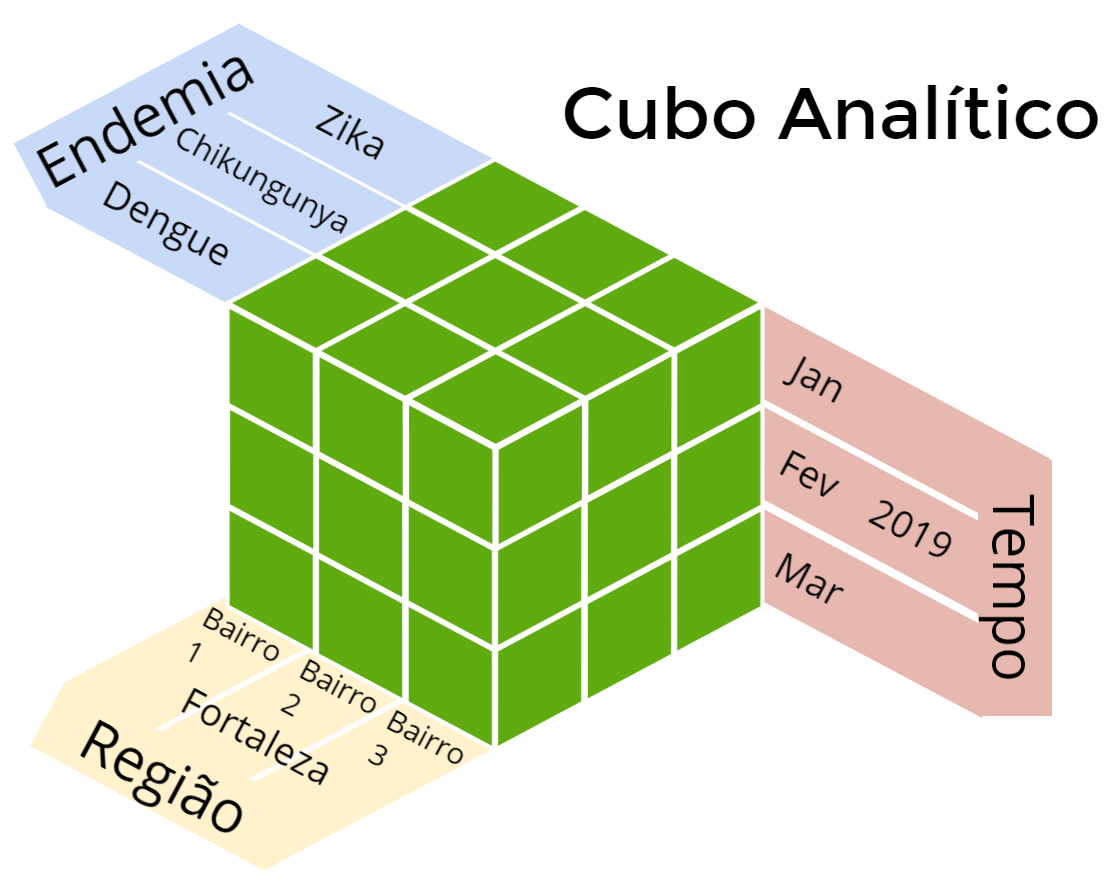
\includegraphics[width=14cm]{figuras/cubo-analitico.png}
	}{
		\Fonte{Elaborado pelo autor}
	}
\end{figure}
\FloatBarrier